\chapter{Algebra}

% !
\section{Quadratic Formula}

\noindent \textbf{The Quadratic Formula} can be used to solve any quadratic 
equation. First, bring a quadratic equation, i.e. $ax^2+bx+c=0$, where $a$, $b$, 
and $c$ are coefficients and $a\neq 0$. Then we plub these coefficients into the 
formula:

\begin{equation*}
  x = \frac{-b \pm \sqrt{b^2-4ac}}{2a}
\end{equation*}


%!
\section{Discriminant}

\noindent Used to determine the number of solutions to the quadratic equation,
$ax^2+bx+c=0$. The formula is:

\begin{equation*}
  b^2-4ac
\end{equation*}


% !
\section{Slope Formula}

\noindent Used to find the slope of a line when you have two points on the line:
$(x_1, y_1); (x_2, y_2)$

\begin{equation*}
  m = \frac{y_2 - y_1}{x_2 - x_1}
\end{equation*}


% !
\section{Point-Slope Form of the Equation of a Line}

\noindent Used to find the equation of a line when given one point $(x_1, y_1)$
and the slope $(m)$.
\begin{equation*}
  y - y_1 = m(x-x_1)
\end{equation*}


% !
\section{Slope Intercept Form of the Equation of a Line}

\noindent Where $m =$ slope and $b =$ y-intercept
\begin{equation*}
  y=mx+b
\end{equation*}


% !
\section{Midpoint Formula}

\noindent Used to find the midpoint of a line segment with endpoints 
$(x_1, y_1)$ and $(x_2, y_2)$
\begin{equation*}
  \left( \frac{x_1 + x_2}{2}, \frac{y_1 + y_2}{2} \right)
\end{equation*}


% !
\section{Distance Formula}

\noindent Used to find the distance between two points: $(x_1, y_1)$ and 
$(x_2, y_2)$
\begin{equation*}
  d = \sqrt{(x_2 - x_1)^2 + (y_2 - y_1)^2}
\end{equation*}


% !
\section{Vertex of a Parabola}

\noindent Given a quadratic formula, $ax^2+bx+c=0$
\begin{equation*}
  \left( -\frac{b}{2a}, f\left(-\frac{b}{2a} \right)\right)
\end{equation*}


% !
\section{Completing the Square}

Completing the square is a technique for rewriting quadratics in the form
$(x+a)^2+b$.\\

\noindent For example, $x^2+2x+3$ can be written as $(x+1)^2+2$. The two 
expressions are totally equivalent, but the second one is nicer to work with in 
some situations.

\begin{framed}
  \noindent \textbf{Example for Completing the Square}\\
  Let's say we are given a quadratic and asked to complete the square:
  \begin{equation*}
    x^2 + 10x + 24 = 0
  \end{equation*}

  \noindent We begin by moving the constant term to the right side of the 
  equation.

  \begin{equation*}
    x^2 + 10x = -24
  \end{equation*}

  \noindent We complete the square by taking half of the coefficient of our $x$
  term, squaring it, and adding it to both sides of the equation. Since the
  coefficient of our $x$ term is 10, half of it would be 5, and squaring it 
  gives us 25.

  \begin{equation*}
    x^2 + 10x + 25 = -24 + 25
  \end{equation*}

  \noindent We can now rewrite the left side of the equation as a squared term.

  \begin{equation*}
    (x+5)^2 = 1
  \end{equation*}

  \noindent Take the square root of both sides.

  \begin{equation*}
    x+5 = \pm 1
  \end{equation*}

  \noindent Isolate $x$ to find the solution(s).

  \begin{equation*}
    x = -5 \pm 1
  \end{equation*}
\end{framed}

\newpage

% !
\section{Pythagorean Theorem}

\noindent Used to find the missing side of a \underline{right} triangle:\\
a = length of side;\\
b = length of side;\\
c = hypotenuse
\begin{equation*}
  a^2+b^2=c^2
\end{equation*}

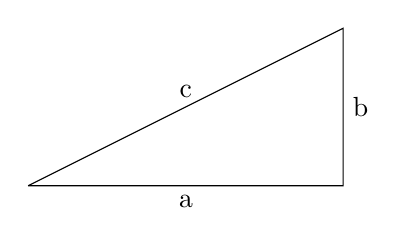
\begin{tikzpicture} 
    \coordinate (a) at (0,0);
    \coordinate (b) at (4,0);
    \coordinate (c) at (4,2);
    \draw (a) -- (b)node[midway, below]{a} -- (c)node[midway,right]{b} -- 
    (a)node[midway,left, above]{c}; % Triangle.
\end{tikzpicture}


% !
\section{Rules of Logarithms}
\noindent Where:\\
$b > 0$ but $b \neq 1$, and \textcolor{red}M, \textcolor{blue}N, and k are real 
numbers but \textcolor{red}M and \textcolor{blue}N must be positive

\begin{framed}
  \noindent General: Common Logarithm
  \begin{equation*}
    \log_{\textcolor{red}{10}} x \rightarrow \log x
  \end{equation*}
  \noindent If the logarithm is using base-10, it is common to drop the number 
  10 because it is understood.
\end{framed}

\begin{framed}
  \noindent General: Natural Logarithm
  \begin{equation*}
    \log_{\textcolor{red}{e}} x \rightarrow \ln x
  \end{equation*}
  \noindent If the logarithm is using base-e, you can replace log base e with 
  just \textcolor{red}{ln}.
\end{framed}

\begin{framed}
  \noindent General: Natural Logarithm evaluated at $e^x$
  \begin{equation*}
    \ln (e^x) = x
  \end{equation*}
  \noindent If the $\ln$ is evaluated at $e^x$ the two undo eachother and it
    becomes just $x$.
\end{framed}

\begin{framed}
  \noindent General: $e$ raised to the Natural Logarithm of $x$
  \begin{equation*}
    e^{\ln x} = x
  \end{equation*}
  \noindent Again, these two functions undo each other and it becomes $x$
\end{framed}

\begin{framed}
  \noindent Rule 1: Product Rule
  \begin{equation*}
    \log_b(\textcolor{red}M \cdot \textcolor{blue}N) 
    = \log_b \textcolor{red}M + \log_b \textcolor{blue}N
  \end{equation*}
  \noindent The logarithm of the product is the sum of the logarithms of the 
  factors.
\end{framed}

\begin{framed}
  \noindent Rule 2: Quotient Rule
  \begin{equation*}
    \log_b \left(\frac{\textcolor{red}M}{\textcolor{blue}N}\right) 
    = \log_b \textcolor{red}M - \log_b \textcolor{blue}N
  \end{equation*}
  \noindent The logarithm of the ratio of two quantities is the logarithm of 
  the numerator minus the logarithm of the denominator.
\end{framed}

\begin{framed}
  \noindent Rule 3: Power Rule 
  \begin{equation*}
    \log_b (\textcolor{red}M^k) = k \cdot \log_b \textcolor{red}M
  \end{equation*}
  \noindent The logarithm of an exponential number is the exponent times the 
  logarithm of the base.
\end{framed}

\begin{framed}
  \noindent Rule 4: Zero Rule 
  \begin{equation*}
    \log_b (1) = 0
  \end{equation*}
  \noindent The logarithm of 1 to any base is always equal to zero. As long as
  $b$ is positive but $b \neq 1$.
\end{framed}

\begin{framed}
  \noindent Rule 5: Identity Rule 
  \begin{equation*}
    \log_b (b) = 1
  \end{equation*}
  \noindent The logarithm of the argument (inside the parenthesis) wherein the 
  argument equals the base is equal to 1.
\end{framed}

\begin{framed}
  \noindent Rule 6: Inverse Property of Logarithm
  \begin{equation*}
    \log_b (b^k) = k
  \end{equation*}
  \noindent The logarithm of an exponential number where its base is the same 
  as the base of the log is equal to the exponent.
\end{framed}

\begin{framed}
  \noindent Rule 7: Inverse Property of Exponent 
  \begin{equation*}
    b^{\log_b (k)}=k
  \end{equation*}
  \noindent Raising the logarithm of a number to its base is equal to the 
  number.
\end{framed}

\begin{framed}
  \noindent Rule 8: Change of Base Formula
  \begin{equation*}
    \log_{\textcolor{blue}b} \textcolor{red}x 
    = \frac{\log_{\textcolor{teal}c} \textcolor{red}x}{\log_{\textcolor{teal}c} 
    \textcolor{blue}b}
  \end{equation*}
  \noindent Where the argument \textbf{\textcolor{red}x} becomes the argument 
  of the numerator logarithm.\\
  The base \textbf{\textcolor{blue}b} becomes the argument of the denominator 
  logarithm.\\
  And the logs in the numerator and denominator have the same base 
  \textbf{\textcolor{teal}c}, the value we chose.
\end{framed} 


% !
\section{Special Factoring Formulas}

\begin{framed}
  \noindent \textbf{Factoring Formula 1:} $(a+b)^2=a^2+2ab+b^2$\\
  \noindent Let us start with the left-hand side of this formula and reach the 
  right-hand side at the end.\\
  \begin{equation*}
    (a+b)^2 = (a+b)(a+b)
  \end{equation*}
  \centerline {Multiply the binomials}
  \begin{equation*}
    = a^2 + ab + ab + b^2
  \end{equation*}
  \begin{equation*}
    =a^2 + 2ab + b^2
  \end{equation*}
\end{framed}

\begin{framed}
  \noindent \textbf{Factoring Formula 2:} $(a-b)^2=a^2-2ab+b^2$\\
  \noindent Let us start with the left-hand side of this formula and reach the 
  right-hand side at the end.\\
  \begin{equation*}
    (a-b)^2 = (a-b)(a-b)
  \end{equation*}
  \centerline {Multiply the binomials}
  \begin{equation*}
    = a^2 - ab - ab + b^2
  \end{equation*}
  \begin{equation*}
    =a^2 - 2ab + b^2
  \end{equation*}
\end{framed}


\begin{framed}
  \noindent \textbf{Factoring Formula 3:} $(a+b)(a-b)=a^2-b^2$\\
  \noindent Let us start with the left-hand side of this formula and reach the 
  right-hand side at the end.\\\\
  \centerline {Multiply the binomials}
  \begin{equation*}
    (a+b)(a-b)=a^2-ab+ba+b^2
  \end{equation*}
  \begin{equation*}
    =a^2-b^2
  \end{equation*}
\end{framed}

\begin{framed}
  \noindent \textbf{Factoring Formula 4:} $x^3+y^3=(x+y)(x^2-xy+y^2)$\\
  \noindent Let us start with the left-hand side of this formula and reach the 
  right-hand side at the end.\\
  \begin{equation*}
    (x+y)(x^2-xy+y^2)
  \end{equation*}
  \begin{equation*}
    =x^3-x^2y+xy^2+x^2y-xy^2+y^3
  \end{equation*}
  \begin{equation*}
    =x^3+y^3
  \end{equation*}
\end{framed}


\begin{framed}
  \noindent \textbf{Factoring Formula 5:} $x^3-y^3=(x-y)(x^2+xy+y^2)$\\
  \noindent Let us start with the left-hand side of this formula and reach the 
  right-hand side at the end.\\
  \begin{equation*}
    (x-y)(x^2+xy+y^2)
  \end{equation*}
  \begin{equation*}
    =x^3+x^2y+xy^2-x^2y-xy^2-y^3
  \end{equation*}
  \begin{equation*}
    =x^3-y^3
  \end{equation*}
\end{framed}


\begin{framed}
  \noindent \textbf{Factoring Formula 6:} $(x+a)(x+b)=x^2+(a+b)x+ab$\\
  \noindent Let us start with the left-hand side of this formula and reach the 
  right-hand side at the end.\\\\
  \centerline {Multiply the binomials}
  \begin{equation*}
    (x+a)(x+b)=x^2+xb+ax+b^2
  \end{equation*}
  \begin{equation*}
    =x^2 + (a + b) x + ab
  \end{equation*}
\end{framed}


\begin{framed}
  \noindent \textbf{Factoring Formula 7:} $(a+b)^3=a^3+b^3+3ab(a+b)$\\
  \noindent Let us start with the left-hand side of this formula and reach the 
  right-hand side at the end.\\
  \begin{equation*}
    (a+b)^3 = (a+b)^2(a+b)
  \end{equation*}
  \begin{equation*}
    =(a^2+2ab+b^2)(a+b)
  \end{equation*}
  \begin{equation*}
    =a^3+2a^2b+ab^2+a^2b+2ab^2+b^3
  \end{equation*}
  \begin{equation*}
    =a^3+b^3+3a^2b+3ab^2
  \end{equation*}
  \centerline{or}
  \begin{equation*}
    a^3+b^3+3ab(a+b)
  \end{equation*}
\end{framed}


\begin{framed}
  \noindent \textbf{Factoring Formula 8:} $(a-b)^3=a^3-b^3-3ab(a-b)$\\
  \noindent Let us start with the left-hand side of this formula and reach the 
  right-hand side at the end.\\
  \begin{equation*}
    (a-b)^3 = (a-b)^2(a-b)
  \end{equation*}
  \begin{equation*}
    =(a^2-2ab+b^2)(a-b)
  \end{equation*}
  \begin{equation*}
    =a^3-2a^2b+ab^2-a^2b+2ab^2-b^3
  \end{equation*}
  \begin{equation*}
    =a^3-b^3-3a^2b+3ab^2
  \end{equation*}
  \centerline{or}
  \begin{equation*}
    a^3-b^3-3ab(a-b)
  \end{equation*}
\end{framed}

\begin{framed}
  \noindent \textbf{Factoring Formula 9:} $(a+b+c)^2=a^2+b^2+c^2+2ab+2bc+2ca$\\
  \noindent Let us start with the left-hand side of this formula and reach the 
  right-hand side at the end.\\
  \begin{equation*}
    (a+b+c)^2 = (a+b+c)(a+b+c)
  \end{equation*}
  \begin{equation*}
    =a^2+ab+ac+ba+b^2+bc+ca+bc+c^2
  \end{equation*}
  \begin{equation*}
    =a^2+b^2+c^2+2ab+2bc+2ca
  \end{equation*}
\end{framed}


\begin{framed}
  \noindent \textbf{Factoring Formula 10:} $x^3+y^3+z^3-3xyz=(x+y+z)(x^2+y^2+z^2-xy-yz-xz)$\\
  \noindent Let us start with the left-hand side of this formula and reach the 
  right-hand side at the end.\\
  \begin{equation*}
    (x+y+z)(x^2+y^2+z^2-xy-yz-xz)
  \end{equation*}
  \begin{equation*}
    = (x^3 + xy^2 + xz^2 - x^2y - xyz - x^2z)
    + (x^2y+y^3+yz^2-xy^2-y^2z-xyz)+(x^2z+y^2z+z^3-xyz-yz^2-xz^2)
  \end{equation*}
  \centerline{Cancel terms}
  \begin{equation*}
    =x^3+y^3+z^3 -3xyz
  \end{equation*}
\end{framed}

